\documentclass{standalone}
\usepackage{tikz}
\usepackage{pgfplots}
\pgfplotsset{width=32cm,height=18cm,compat=1.3}
\pgfplotsset{every tick label/.append style={font=\Huge}}
\usepackage{filecontents}

\usetikzlibrary{patterns}

\definecolor{citrine}{rgb}{0.89, 0.82, 0.04}

\begin{document}
	\centering
		\vspace{1.5em}
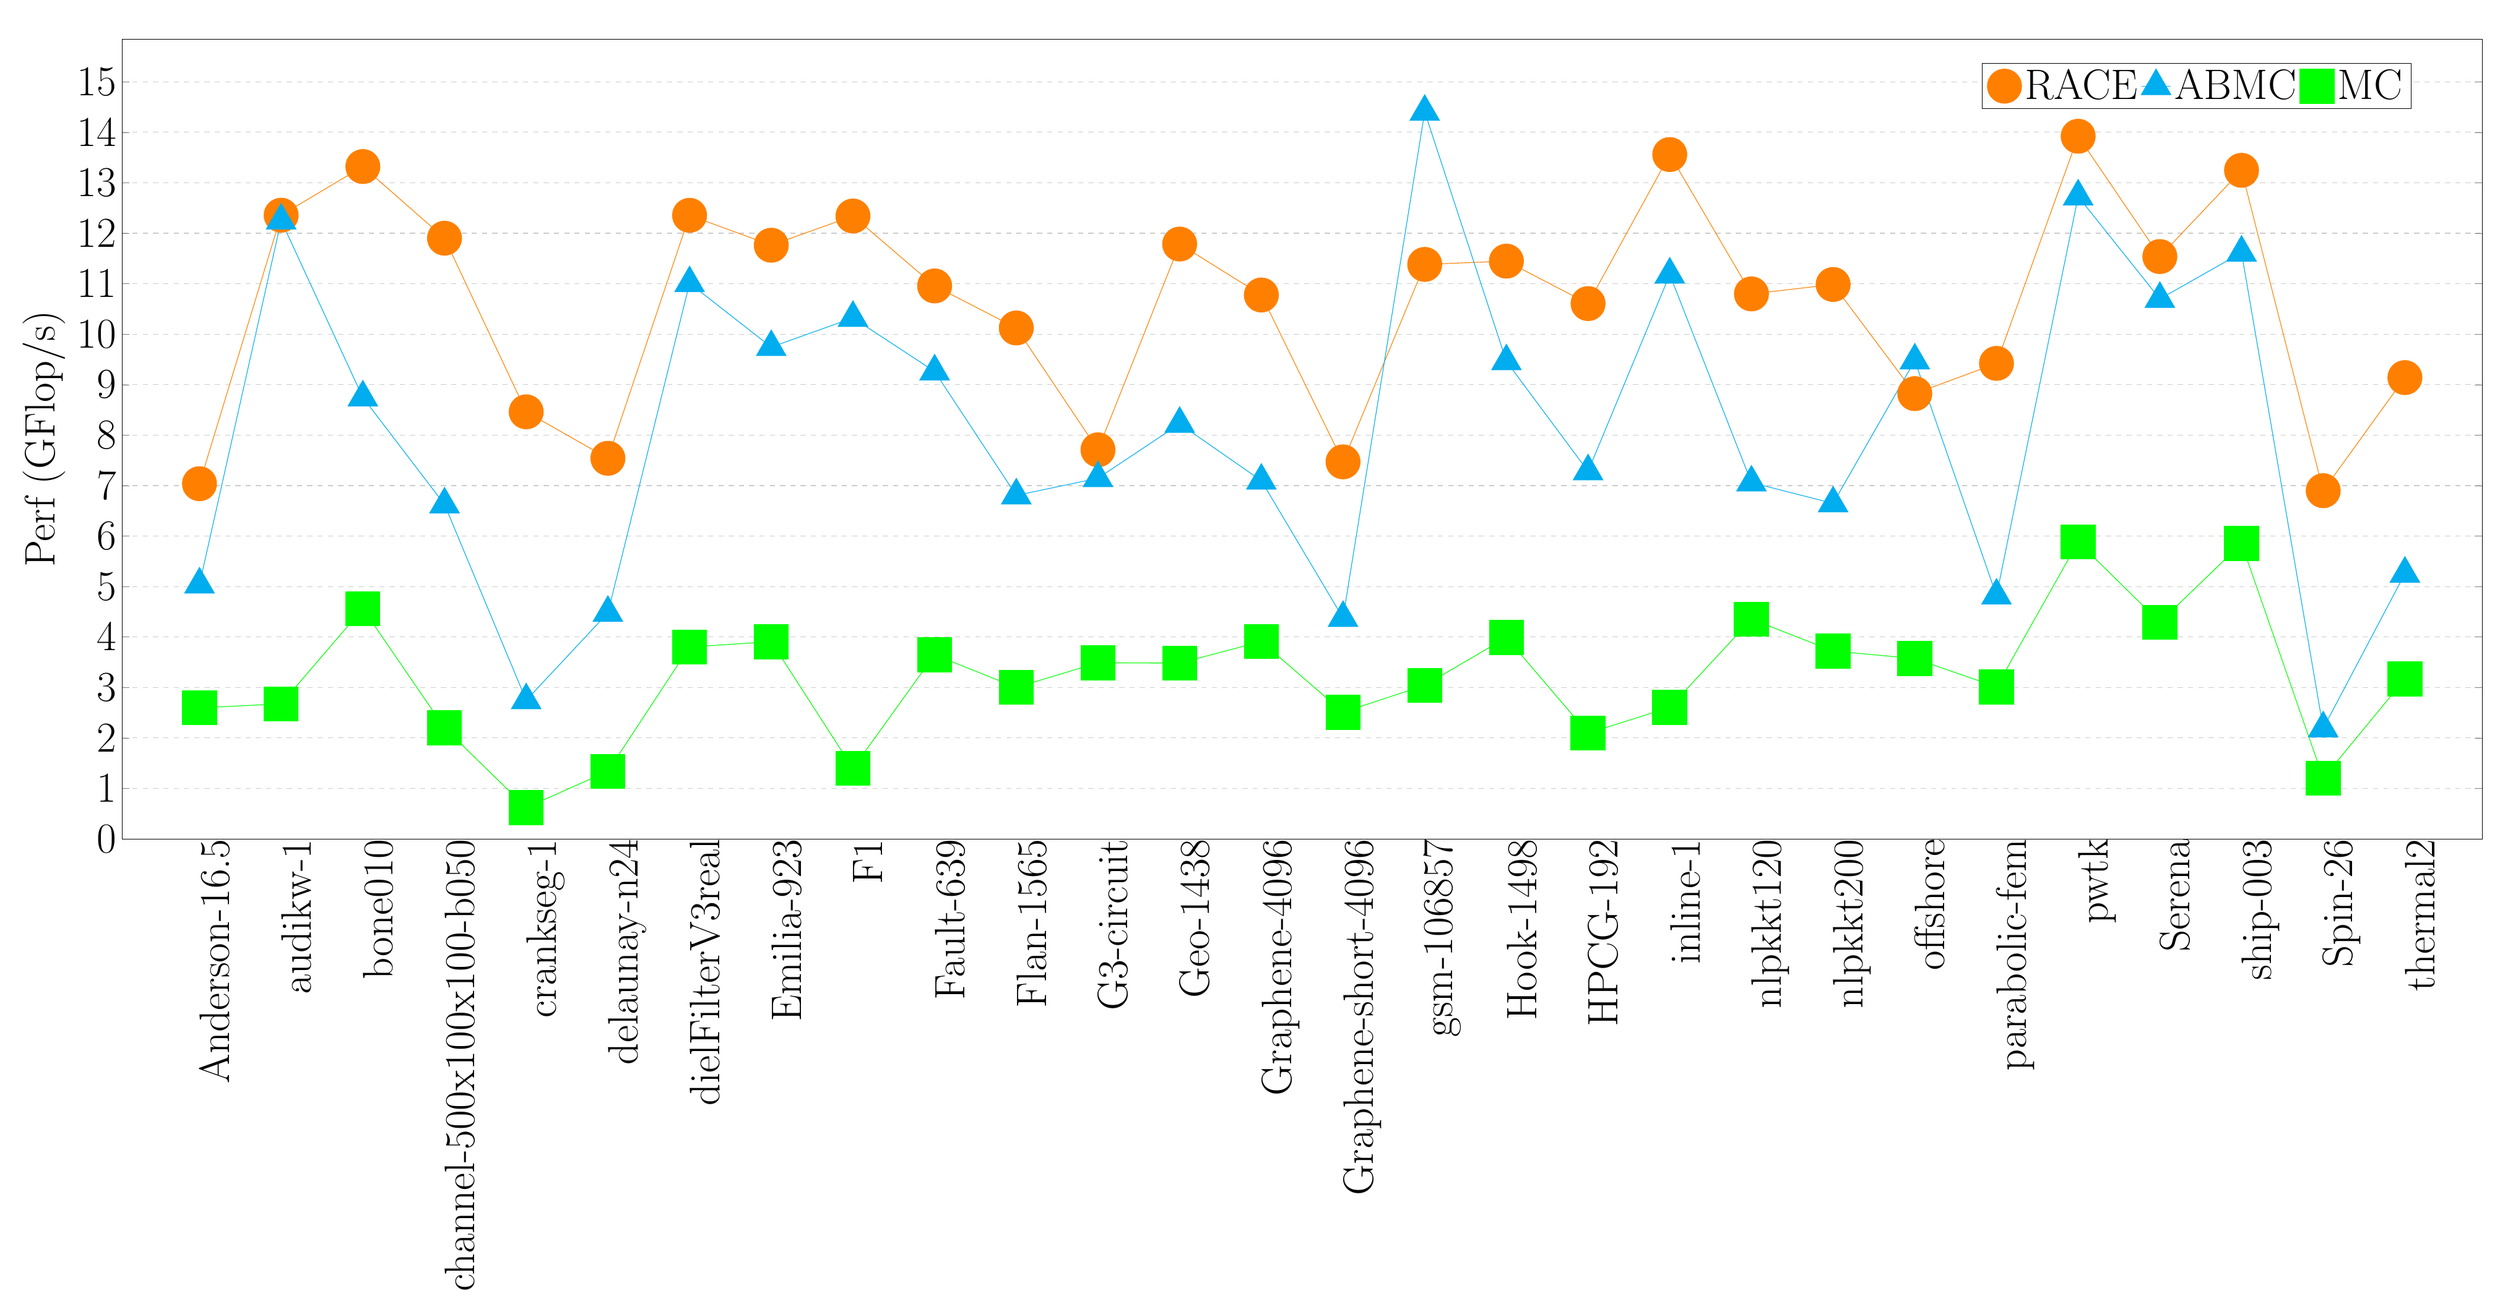
\begin{tikzpicture}
		%	\node at (13.25,15) {\LARGE{}};
			\begin{axis}[
		%	xmin=0.25, xmax=7.25,
			ymin=0, %ymax=3.25,
			xtick={1, 2, 3, 4, 5, 6, 7, 8, 9, 10, 11, 12, 13, 14, 15, 16, 17, 18, 19, 20, 21, 22, 23, 24, 25, 26, 27, 28},
		%	ytick={0,0.5,1,1.5,2,2.5,3},
			xticklabels={Anderson-16.5, audikw-1, bone010, channel-500x100x100-b050, crankseg-1, delaunay-n24, dielFilterV3real, Emilia-923, F1, Fault-639, Flan-1565, G3-circuit, Geo-1438, Graphene-4096, Graphene-short-4096, gsm-106857, Hook-1498, HPCG-192, inline-1, nlpkkt120, nlpkkt200, offshore, parabolic-fem, pwtk, Serena, ship-003, Spin-26, thermal2},
			width  = 50cm,
			height = 18cm,
			major x tick style = transparent,
			%	minor ytick={1, 5, 10, 15, 20, 25, 30 ,35,40},
			grid = minor,	
			%add_bar_commands
			ymajorgrids = true,
			grid style={dashed, gray!40},
			ylabel = {\Huge{Perf (GFlop/s)}},
		%	symbolic x coords={Graphene-2048-2048, Graphene-4096-4096, Spin-24-24-24},
			x tick label style={rotate=90, anchor=north east, inner sep=0mm, font={\Huge}},
			tick label style={font={\Huge}},
			scaled y ticks = false,
			enlarge x limits=0.035,
			legend cell align=left,
			legend style={font=\Huge},
			legend columns=-1,
			legend style={
				%at={(1,1.05)},
				%anchor=south east,
				%column sep=1ex,
				legend pos=north east
			},
			%spl_legend_code
			title= {\Huge\scalebox{1.5}{{}}}
			]

\addplot[mark=*, mark size=10pt, mark options={orange}, draw=orange , y filter/.code={\pgfmathparse{\pgfmathresult*1000}\pgfmathresult}] plot coordinates{(1,.00703714324324324324) (2,.01235745643564356435) (3,.01332161089108910891) (4,.01190178823529411764) (5,.00846153173076923076) (6,.00754096078431372549) (7,.01235514257425742574) (8,.01176216542056074766) (9,.01234152574257425742) (10,.01095599908256880733) (11,.01012329097744360902) (12,.00770854563106796116) (13,.01178579117647058823) (14,.01077660594059405940) (15,.00747042970297029702) (16,.01138242400000000000) (17,.01144760194174757281) (18,.01060615727272727272) (19,.01355900900000000000) (20,.01079820000000000000) (21,.01098451666666666666) (22,.00882238543689320388) (23,.00942133689320388349) (24,.01392203725490196078) (25,.01153803636363636363) (26,.01324681470588235294) (27,.00689933064516129032) (28,.00913995148514851485)};
\addplot[mark=triangle*, mark size=10pt, mark options={cyan}, draw=cyan , y filter/.code={\pgfmathparse{\pgfmathresult*1000}\pgfmathresult}] plot coordinates{(1,.00504018611111111111) (2,.01225110000000000000) (3,.00874625912408759124) (4,.00662585486725663716) (5,.00274606933333333333) (6,.00447836904761904761) (7,.01100942596153846153) (8,.00974393109243697478) (9,.01032287327586206896) (10,.00926169312977099236) (11,.00680515838150289017) (12,.00714632857142857142) (13,.00822354924242424242) (14,.00709740260869565217) (15,.00437658761904761904) (16,.01440536547619047619) (17,.00946195964912280701) (18,.00728254649122807017) (19,.01118077818181818181) (20,.00705996071428571428) (21,.00664720964912280701) (22,.00947787191011235955) (23,.00482023351063829787) (24,.01272802075471698113) (25,.01069810198019801980) (26,.01161557254901960784) (27,.00218936637168141592) (28,.00525437852348993288)};
\addplot[mark=square*, mark size=10pt, mark options={green}, draw=green , y filter/.code={\pgfmathparse{\pgfmathresult*1000}\pgfmathresult}] plot coordinates{(1,.00259613511450381679) (2,.00267594537815126050) (3,.00456334028776978417) (4,.00220035500000000000) (5,.00062049233333333333) (6,.00133974041095890410) (7,.00380282407407407407) (8,.00390729727891156462) (9,.00139696343283582089) (10,.00364767843137254901) (11,.00300092588832487309) (12,.00348970655737704918) (13,.00348306535947712418) (14,.00391036771653543307) (15,.00250906140350877192) (16,.00304297926829268292) (17,.00399057686567164179) (18,.00209408897058823529) (19,.00260585407407407407) (20,.00435293902439024390) (21,.00372281129032258064) (22,.00357235172413793103) (23,.00301229644670050761) (24,.00588453166666666666) (25,.00429262689075630252) (26,.00585221359223300970) (27,.00120325038759689922) (28,.00316779933774834437)};
	%addplot cmd

	\legend{RACE, ABMC, MC}

	\end{axis}			
\end{tikzpicture}

\end{document}

